\section{Concept: conventional joints}
\label{Concept: conventional joints}
Three concepts are designed based on conventional joints, meaning that no flexures are used. These concepts are presented and evaluated after which one concept is selected based on a selection table.
%\subsection{Hysteresis}
%In precision products, joined parts must maintain their relative position. If under either thermal or mechanical load shift takes place most certainly the relative position in the unloaded state is also changed. The phenomenon responsible for this is hysteresis or virtual backlash. The virtual play in a simple model is described by $S_v = \frac{2W}{c}$ where $W$ is the friction and {c} the stiffness.


\subsection{Degrees of freedom}
First of all an overview is made of the different ways to enable motion in the degrees of freedom. A division is made between translational degrees of freedom and rotational degrees of freedom.
\subsubsection{Translational degrees of freedom}
As stated in section \ref{requirementandassumptions} the design has two translational degrees of freedom. In this subsection all the possibilities that a conventional design offers with regards to translational movement are evaluated. \\\\
The most common solution for translation movement is a linear bearing, these bearings exactly constrain 5 degrees of freedom and allow only translational movement. A more advanced version of the linear bearing is an H-drive. An H-drive makes use of three linear bearings which results in an increased stiffness however over-constraining the design.  \\
Another solution for translational movement uses the idea of a column press, this type of guidance is commonly used in high load application but can also be used for this application. \\
A spindle can also be used to obtain a translational movement. This option however results in a high amount of hysteresis and requires a large force to actuate. 


%\begin{enumerate}
%    \item A linear bearing. These types of bearings constraint 5 degrees of freedom and allow only translational movement. 
%    \item An H-drive, this is a commonly used linear drive in precision mechanics. 
%    \item A column press design. This design allows for only one translational degree. Usually these types of constructions are used in high load application instead of precision mechanisms.
%\end{enumerate}
\begin{table}[h] \centering \caption{Translational DOF's: solution overview} \label{tab:transsolutions}
\begin{tabular}{p{3cm}|p{3cm}p{3cm}p{3cm}p{3cm}}
Translational solution   & Linear bearing \cite{lineartrans} & H-drive \cite{lecturesheets} & Column press \cite{TOXPRESSOTECHNIK4PRESSOTECHNIK} & Spindle\\ \hline
Figure for clarification &     
    \begin{minipage}{3cm}
      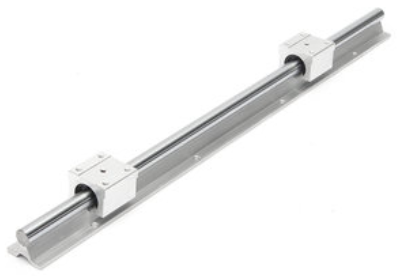
\includegraphics[width=\linewidth]{images/linear.png}
    \end{minipage} 
    &     
    \begin{minipage}{3cm}
      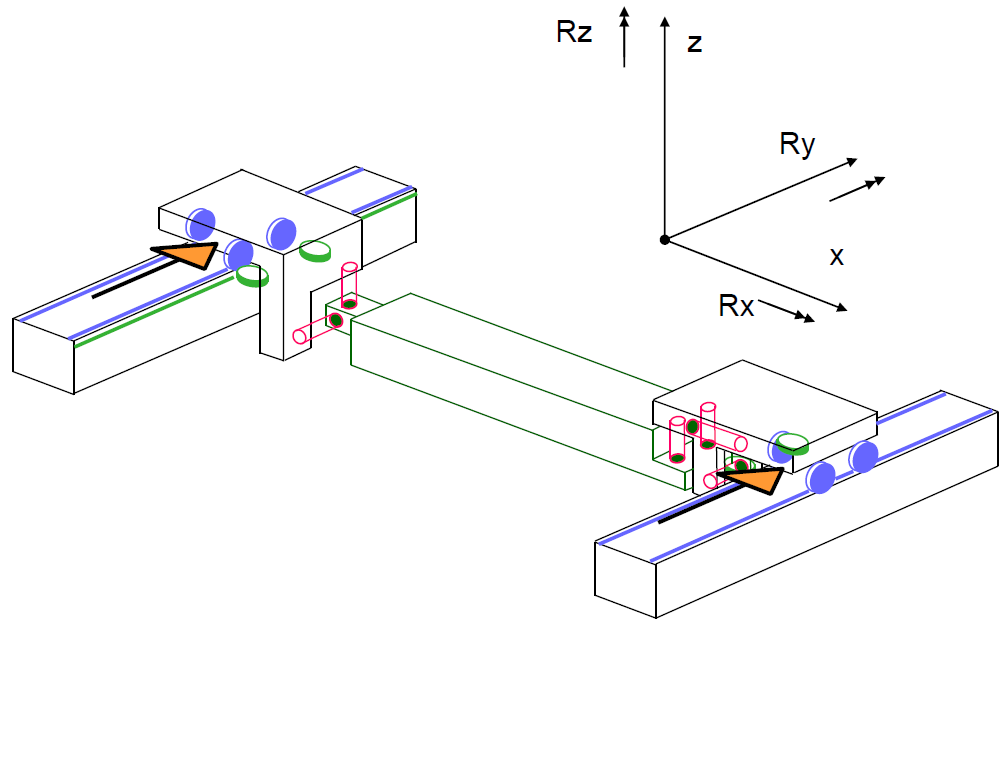
\includegraphics[width=\linewidth]{images/Hdrive}
    \end{minipage} 
    &     
    \begin{minipage}{3cm}
      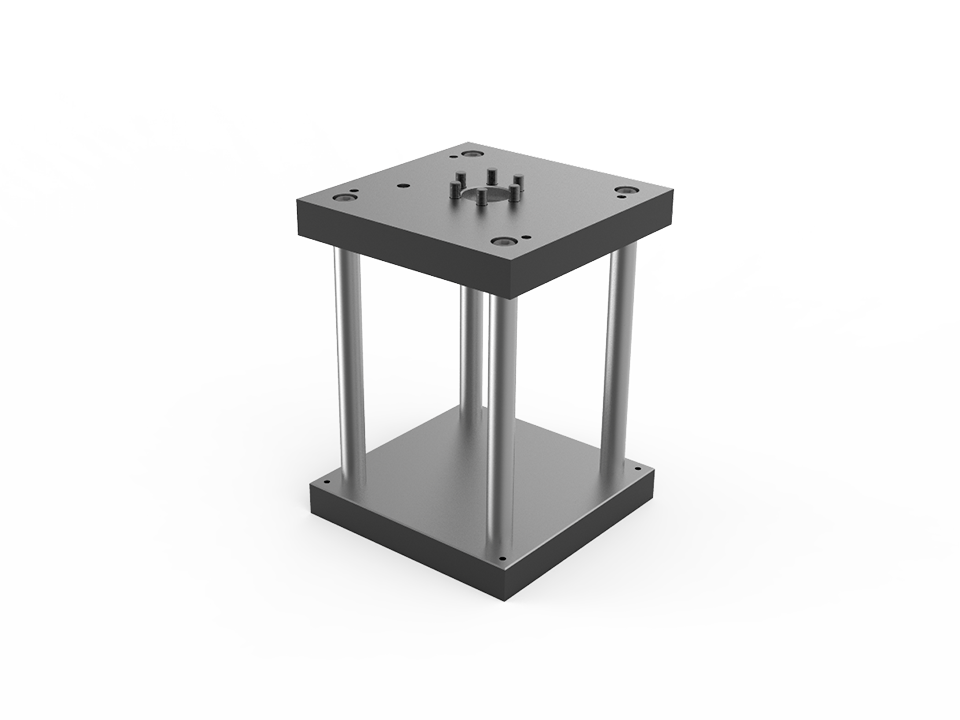
\includegraphics[width=\linewidth]{images/column_press.png}
    \end{minipage}
    &
    \begin{minipage}{3cm}
      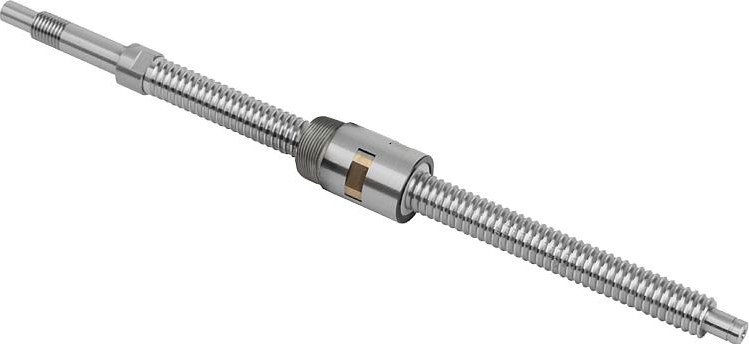
\includegraphics[width=\linewidth]{images/spindle.png}
    \end{minipage} \\ \hline
Advantages               & Exact constraint & Stiff & High loads & Relatively accurate \\ \hline
Disadvantages            & None & Vulnerable to misalignment & Over constraint & Low translational speed  \\ 
\end{tabular}
\end{table}
%\subsubsection{Selection}
%\label{translationalselection}
%Taking into account the advantages and disadvantages of the various option a selection can be made. It is clear that a column press set-up is unsuitable for the precision mechanisms application as the forces are significantly smaller than optimal and the over constrained design would require precise engineering. An h-drive setup is beneficial for application where a high stiffness is required. In the current application a conventional linear bearing is sufficient for the translation degrees of freedom.

\subsubsection{Rotational degrees of freedom}
The design requires two rotational degrees of freedom that have a range of motion of 90$^o$ as stated in section \ref{requirementandassumptions}. Non-flexure based designs have several alternatives to obtain this range of motion. \\\\
The most used solution for a rotational movement is the use of a roller bearing. Several types of roller bearings are obtainable, conventional bearing using balls, air bearings using a small film of pressurised fluid and magnetic bearings using magnetic levitation. \\
Ball joints are able to obtain both a horizontal and vertical rotation. These joints are however more difficult to actuate. \\
Another option for rotational movement is the use of a worm drive. This concept uses a worm screw in combination with a worm drive to obtain a 90 degree rotation. 
%\begin{enumerate}
%    \item A conventional roller bearing. This bearing uses two races, which are the bearing rings, between which several balls roll. These races feature grooves that are shaped such that the ball fits slightly loose. The conventional roller bearing can be further divided in radial and axial.
%    \item An air bearing, which is more advanced. These bearings use a thin film of pressurised gas instead of balls. The use of pressurised gas as interface between the two surfaces allows for a low friction bearing. Next to this lower friction air bearings also have the advantage that it allows for non contact usage, therefore neglecting problems such as friction, wear and lubricant handling. 
%    \item Magnet bearing use magnetic levitation to support the load. The rotating shaft is levitated allowing a very low friction and no mechanical wear. This type of bearing supports the highest speed of all kinds of bearings. Downside of this type is that most of the time active magnetic bearing are used, meaning that a constant input power is required. Next to this magnetic bearing tyipically require a back-up bearing in the case of power or control system failure. 
%\end{enumerate}

\begin{table}[h] \centering \caption{Rotational DOF's: solution overview} \label{tab:rotationsolutions}
\begin{tabular}{p{4cm}|p{4cm}p{4cm}p{4cm}}
Rotational solution         & Roller bearing \cite{123RFBall54180420.} & Air bearing \cite{NELSONAIRAirAir} & Magnetic bearing \cite{magneticbearing} \\ \hline
Figure for clarification    & 
    \begin{minipage}{4cm}
      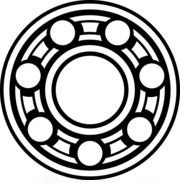
\includegraphics[width=\linewidth]{images/Ball_bearing2.jpg}
    \end{minipage} 
    &     
    \begin{minipage}{4cm}
      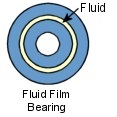
\includegraphics[width=\linewidth]{images/airbearing.jpg}
    \end{minipage} 
    &     
    \begin{minipage}{4cm}
      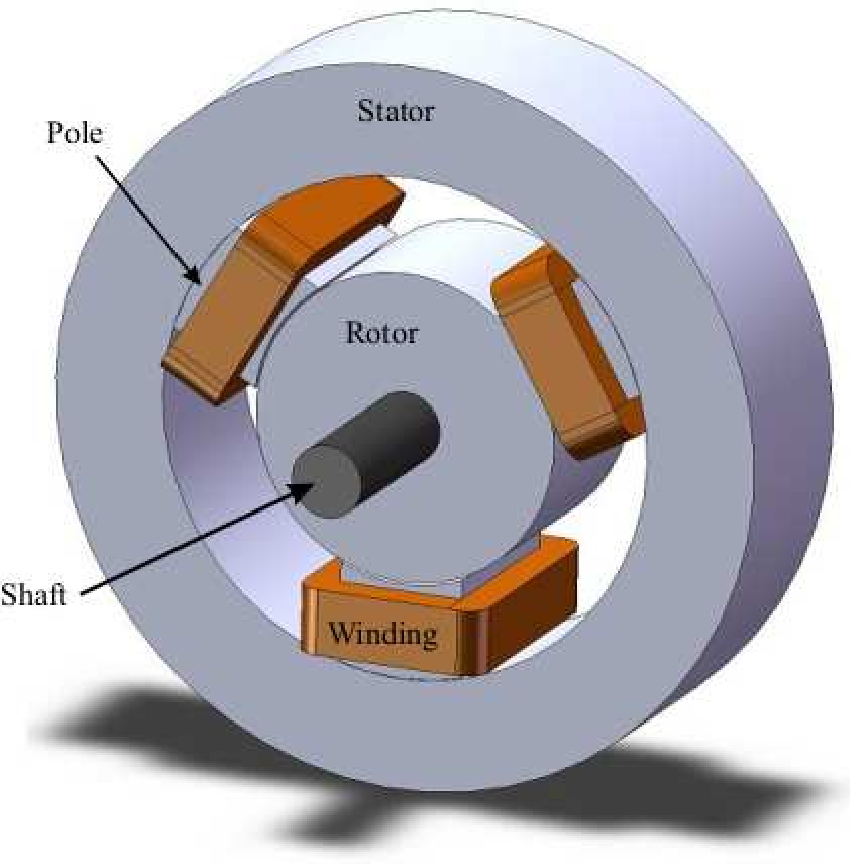
\includegraphics[width=\linewidth]{images/magnetic_bearing.png}
    \end{minipage} \\ \hline
Maximum angle               & 360\degree & 360\degree   & 360\degree  \\ \hline
Advantages                  & Cheap and widely available & Non-contact & No friction \\ \hline
Disadvantages               &  Wear and tear & Requires perfect geometry  & Large size  \\ 
\end{tabular}
\end{table}
%\subsubsection{Selection}
%\label{rotationalselection}
%Three types of bearings are proposed for the rotational degrees of freedom. The bearing will be selected based on efficiency and volume. A magnetic bearing has the lowest amount of friction however there are some drawbacks to this type, due to the required back-up bearing and constant power input the volume required for this bearing is significantly larger than the others. The available volume is limited, therefore a magnetic bearing won't be used. Roller and air bearings are both suitable for the proposed application. However due to the non-contact movement in the air bearing no wear and tear will occur which will be beneficial, therefore air bearings will be used for the rotational degrees of freedom. 

\subsection{Concept evaluation}
Knowing all the different ways to achieve the desired degrees of freedom several concepts have been made. In this section the different concepts are presented, visualised and evaluated based on several factors.
\subsubsection{Concept 1: Translational frame}
The first concept makes use of a translational table to cover the range of the disk and a double rotational cube to achieve the rotational position. This concept is shown visually in figure \ref{fig:convential_concept_1}. In this figure the translational table is shown to the left, this table makes use of several H-drive t


\begin{figure}[!h]
    \centering
    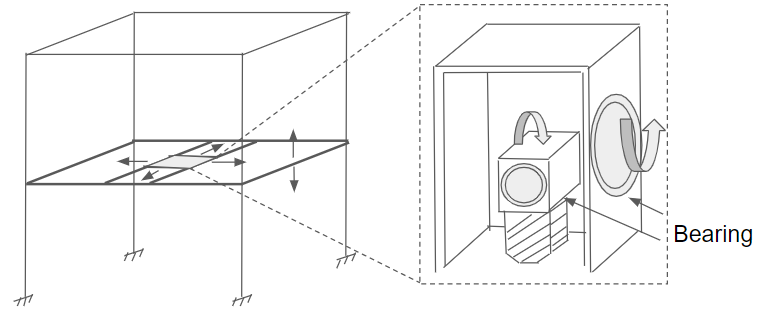
\includegraphics[width=0.6\textwidth]{images/Conventional_concept_1.PNG}
    \caption{Translational table concept}
    \label{fig:convential_concept_1}
\end{figure}



\subsubsection{Concept 2: Crane}




\subsubsection{Concept 3: Delta robot}


\subsection{Concept selection}
%As mentioned in sections \ref{rotationalselection} and \ref{translationalselection} the conventional concept will be based on linear bearings in combination with rotational air bearings. In figure \ref{fig:conventional_concept} a sketch of the concept can be seen. In this concept the first body can rotate 90 degrees, the second body can translate 1 mm, the third body can translate 10 mm and the fourth body can rotate 45 degrees. 
%\begin{figure}[h]
%    \centering
%    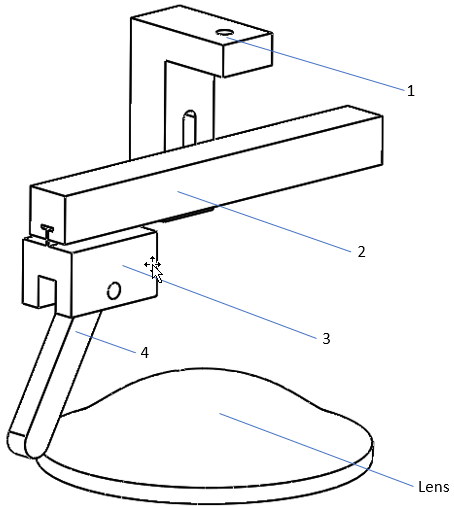
\includegraphics[width=0.5\textwidth]{images/conventional_concept.png}
%    \caption{A sketch of the conventional concept}
%    \label{fig:conventional_concept}
%\end{figure}

